    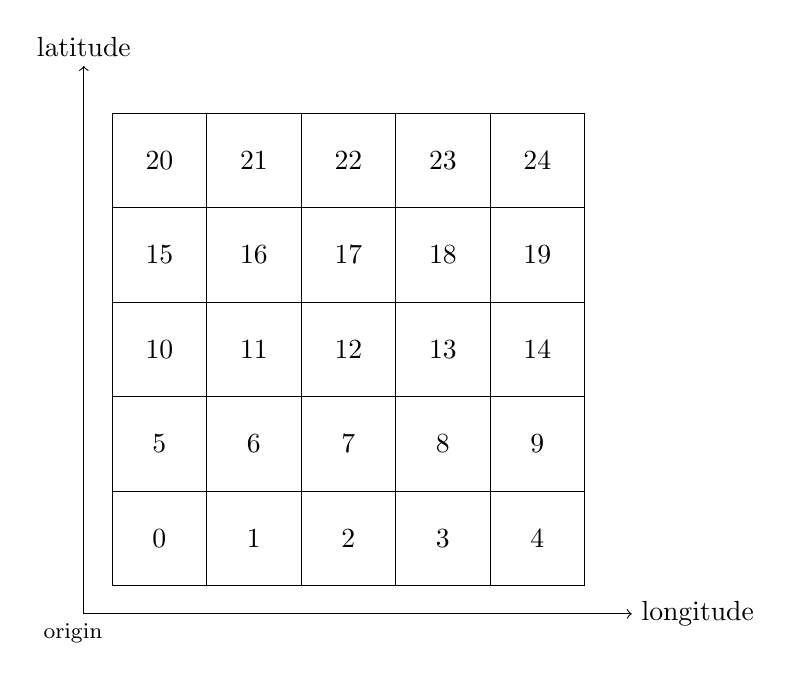
\begin{tikzpicture}[scale=1.2]
        \def\side{5}
        \foreach \row in {0,...,4} {
            \foreach \col in {0,...,4} {
                \pgfmathtruncatemacro{\idx}{\row * \side + \col}
                \draw (\col, \row) rectangle (\col+1, \row+1);
                \node at (\col+0.5, \row+0.5) {\idx};
            }
        }
        % Axis labels
        \draw[->] (-0.3, -0.3) -- (5.5, -0.3) node[right] {longitude};
        \draw[->] (-0.3, -0.3) -- (-0.3, 5.5) node[above] {latitude};
        % Origin label
        \node[below left] at (0, -0.3) {\footnotesize origin};
    \end{tikzpicture}